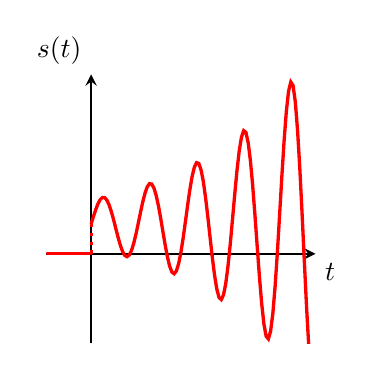
\begin{tikzpicture}
    \tikzstyle{signal}=[very thick,red,domain=-2:0, samples=101]
    \begin{axis}
    [	ticks=none,
        axis line style = thick,
        height=5cm,
        width=5cm,
        axis x line=center,
        axis y line=center,
        xmin=-2,
        xmax=10,
        ymin=-3,
        ymax=6.0,
        xlabel={$t$},
        ylabel={$s(t)$},
        xlabel style={below right},
        ylabel style={above left},
    ]
    \addplot[signal,domain=-2:0] {0};
    \addplot[signal,domain=0:10] {0.8*sin(3*deg(x))*exp(0.2*x)+1};
    \draw[dotted,very thick,red] (axis cs:0,0) -- (axis cs:0,1);
    \end{axis}
\end{tikzpicture}
